%%%%%%%% Klassen-Optionen
\documentclass[12pt,a4paper]{scrartcl}

%%%%%%%% PAKETE: unverzichtbare Pakete mit Einstellungen
\usepackage[left=2.5cm, right=2cm, top=3cm, bottom=3cm, a4paper]{geometry} %Seitenrände
\usepackage[utf8x]{inputenc} % utf8-Kodierung und direkte Eingabe von Sonderzeichen
\usepackage{fixltx2e} % Verbessert einige Kernkompetenzen von LaTeX2e

%%%%%%%% PAKETE: AMS-Pakete
\usepackage{amsmath} % Mathe-Erweiterung
\usepackage{amsfonts} % Schrift-Erweiterung
\usepackage{amssymb} % Sonderzeichen-Erweiterung

%%%%%%%% PAKETE: Sonstiges
\usepackage[colorlinks, citecolor=black, filecolor=black, linkcolor=black, urlcolor=black]{hyperref} % Links
\usepackage{wrapfig} % ausgeklügekte Floatumgebung
\usepackage{float} % normale Floatumgebung
\restylefloat{figure} % ermöglicht die Verwendung von "H" (ist noch stärker als "h!")
\usepackage[small,it,singlelinecheck=false]{caption} % Bildunterschriften formatieren
\usepackage{multirow} % ermöglich Verbinden von Tabellenzeilen
\usepackage{multicol} % ermöglicht Spalten
\usepackage{fancyhdr} % ermöglicht Kopf- und Fußzeilen
\usepackage{graphicx} % Einbinden von Bildern möglich
\usepackage{units} % Einheiten
\usepackage{subcaption}

%%%%%%%% DEFINITIONEN: Titelseite
\author{April Cooper, Patrick Kreissl und Sebastian Weber}
\title{Worksheet 6: Finite-Size Scaling and the Ising Model}
\publishers{University of Stuttgart}
\date{\today}

%%%%%%%% ANPASSUNGEN: Kopf-und Fußzeile
\fancypagestyle{plain}{} % redefine the plain pagestyle to match the fancy layout
\pagestyle{fancy} % aktiviere eigenen Seitenstil
\fancyhf{} % alle Kopf- und Fußzeilen bereinigen
\fancyhead[L]{Worksheet 6: Finite-Size Scaling and the Ising Model}
\fancyhead[R]{\today}
\renewcommand{\headrulewidth}{0.6pt} % obere Trennlinie
\fancyfoot[L]{April Cooper, Patrick Kreissl und Sebastian Weber}
\fancyfoot[R]{Page \thepage}
\renewcommand{\footrulewidth}{0.6pt} % untere Trennlinie

%%%%%%%% ANPASSUNGEN: Absätze
\setlength{\parindent}{0em} % keine Absatzeinzüge
\setlength{\parskip}{0em} % Absatz-Abstand

%%%%%%%% ANPASSUNGEN: Abbildungsverzeichnis
\usepackage{tocloft} % Zum Anpassen der Verzeichnisse
\renewcommand{\cftfigpresnum}{Abb. }
\renewcommand{\cfttabpresnum}{Tab. }
\renewcommand{\cftfigaftersnum}{:}
\renewcommand{\cfttabaftersnum}{:}
\setlength{\cftfignumwidth}{2cm}
\setlength{\cfttabnumwidth}{2cm}
\setlength{\cftfigindent}{0cm}
\setlength{\cfttabindent}{0cm}

%%%%%%%% SONSTIGES
\usepackage{pdfpages}
\usepackage{pgf}

% NÜTZLICH: http://truben.no/latex/table/

% Anfang des eigentlichen Dokuments
\begin{document}

\maketitle
\tableofcontents
\newpage

% =============== Section ============
\section{Finite Size Scaling}

\subsection{Determinig $T_\text{C}$}

In this task the Binder parameter $ U = 1 - \frac{1}{3} <\mu^4>/<\mu^2>^2$ was implemented. The resulting plot of the Binder parameter over the Temperature for different L can be seen below:

\begin{figure}[H]
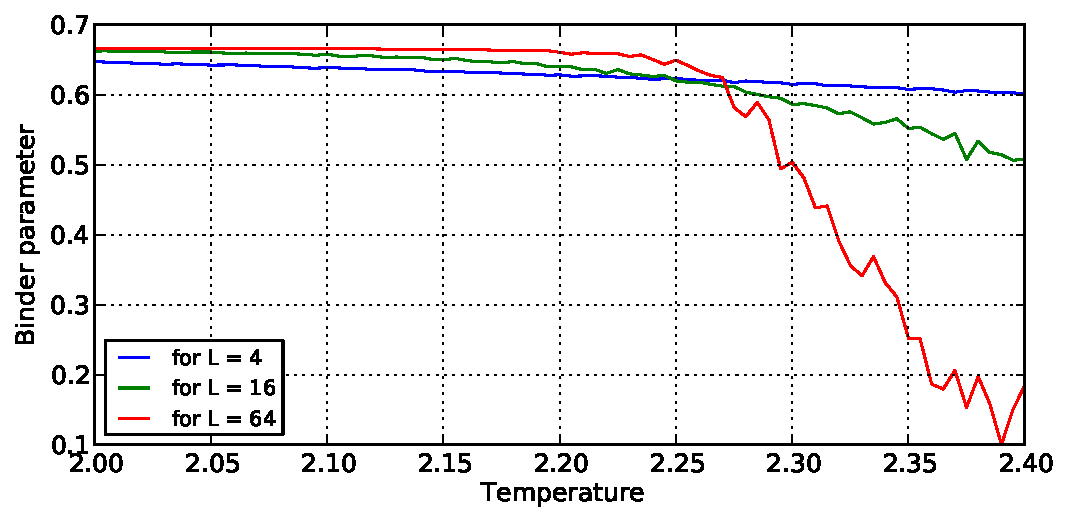
\includegraphics[width=16.0cm]{../plots/2binder_01.pdf}
\caption{Plot of the Binder parameter for different lattice sizes L. From the intersection point of the different curves the critical Temperature can be determined as $T_\text{C} = 2.27 K$. In order to get a good result a 100000 sweeps and a temperature step size of $\Delta t = 0.005$ K were used.}
\end{figure}

\subsection{Estimating $\beta_\text{m}$}

Here we performed different simulations at $T_\text{C} = 2.27 K$ were performed for $L \in \lbrace 8, 16, 32, 64, 128 \rbrace$. The resulting plot of the magnetization $M$ over $L$ is as follows:

\begin{figure}[H]
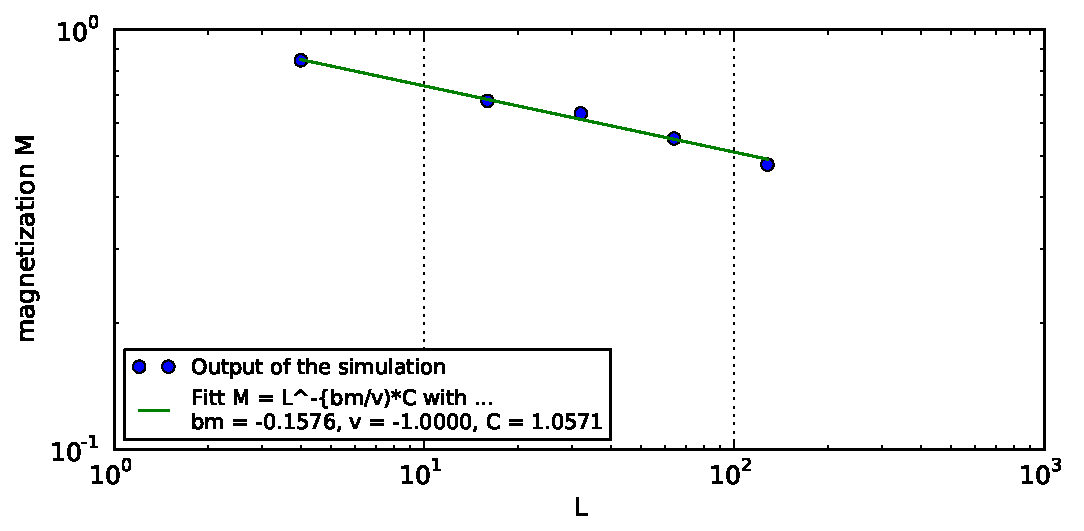
\includegraphics[width=16.0cm]{../plots/3beta_01.pdf}
\caption{Plot of the magnetization $M$ over $L$ with double logarithmic scale. From the linear fit through the computet magnetizations $\beta_\text{m}$ can be determined as -0.1576.}
\end{figure}

The formula which connects the magnetization $M$, lattice size $L$ and $\beta_\text{m}$ is the following:
\begin{equation}
	M = L^{-\beta_\text{m}/\nu}
\end{equation}
It was also used in order to get a value for $\beta_\text{m}$ from the plot.

\end{document}


% =============== Comments ============
\begin{comment}
\verb{x_init {}}

\begin{figure}[H]
	\resizebox{1\textwidth}{!{\input{../plots/NAME.pgf}}
	\caption{CAPTION}\label{fig:NAME}
\end{figure}
\end{comment}
